\documentclass{article}
\usepackage{tikz}
\usepackage{amsmath}
\usepackage{bm}  % put in preamble
\usepackage{empheq}
\usepackage{graphicx}
\usepackage[T1]{fontenc}   % Use T1 font encoding (supports Polish diacritics)
\usepackage[utf8]{inputenc} % Allows UTF-8 encoded Polish letters
\usepackage{url}

\usetikzlibrary{arrows.meta,calc,decorations.pathreplacing}

\title{Symulacja ruchu pojazdu}
\author{v4m3rrr}

\graphicspath{{images/}}

\begin{document}
	\maketitle
	\tableofcontents
	\newpage
	
	\section{Kinematyka pojazdu}
	
	Rozważmy ciało sztywne $M$ poruszające się ruchem dowolnym względem układu odniesienia $Ox'y'z'$, który sam porusza się względem stałego układu odniesienia $O_1xyz$. W tym kontekście punkt $O_1$ może reprezentować środek linii mety, chociaż w ogólności może być dowolnym stałym punktem w przestrzeni. Oznaczamy przez $O$ środek mas pojazdu, a przez $O'x''y''z''$ układ związany z określonym elementem pojazdu. Rysunek \ref{fig:rigid_body} ilustruje ogólny ruch pojazdu \cite{Leyko}.
	
	\begin{figure}[h!]
		\centering
		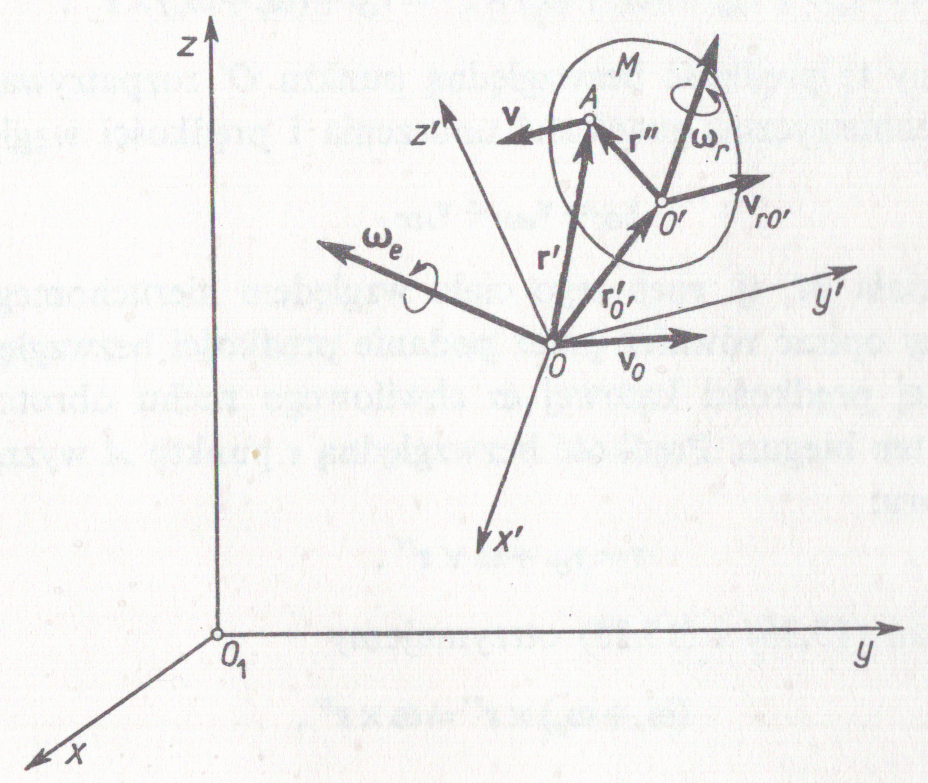
\includegraphics{motion_rigid_body.png}
		\caption{Ogólny ruch ciała sztywnego względem stałych i ruchomych układów odniesienia \cite{Leyko}.}
		\label{fig:rigid_body}
	\end{figure}
	
	Prędkość punktu na ciele sztywnym w stałym układzie odniesienia $O_1xyz$ można wyrazić jako:
	\begin{align}
		\vec{v} = \vec{v}_0 + \vec{\omega}e \times \vec{r'} + \vec{v}{r_0'} + \vec{\omega}_r \times \vec{r''},
	\end{align}
	gdzie:
	\begin{itemize}
		\item $\vec{v}_0$ jest prędkością początku ruchomego układu $Ox'y'z'$ względem stałego układu $O_1xyz$,
		\item $\vec{\omega}e$ jest prędkością kątową ruchomego układu $Ox'y'z'$,
		\item $\vec{r'}$ jest wektorem położenia punktu $A$ względem początku ruchomego układu $O$,
		\item $\vec{v}{r_0'}$ jest prędkością ruchomego układu $O'x''y''z''$ względem ruchomego układu $Ox'y'z'$,
		\item $\vec{\omega}_r$ jest prędkością kątową ruchomego układu $O'x''y''z''$,
		\item $\vec{r}''$ jest wektorem położenia punktu $A$ względem układu $O'x''y''z''$.
	\end{itemize}
	
	Podobnie, wektor położenia punktu $A$ w stałym układzie odniesienia $O_1xyz$ jest następujący:
	\begin{align}
		\vec{r} = \overrightarrow{O_1O} + \vec{r}'{O'} + \vec{r}'',
	\end{align}
	gdzie:
	\begin{itemize}
		\item $\overrightarrow{O_1O}$ jest wektorem położenia środka mas $O$ względem stałego układu $O_1xyz$,
		\item $\vec{r}'{O'}$ jest wektorem położenia punktu $O'$ względem ruchomego układu $Ox'y'z'$,
		\item $\vec{r}''$ jest wektorem położenia punktu $A$ względem układu $O'x''y''z''$.
	\end{itemize}
	
	\section{Model koła}
	
	Zakładając, że koło ma charakterystykę częściowo sprężystą, natomiast nawierzchnia jest doskonale sprężysta (uwzględniając tylko asfalt i beton), strata energetyczna wynikająca z pracy opony (histereza) wynosi:
	\begin{align}
		\Delta A = A_1 - A_2,
	\end{align}
	gdzie:
	\begin{itemize}
		\item $\Delta A$ – strata energetyczna (histereza),
		\item $A_1$ – praca włożona przy obciążeniu opony,
		\item $A_2$ – praca zwracana przy odciążaniu opony.
	\end{itemize}
	
	Przy tak przyjętej charakterystyce zawsze zachodzi nierówność $\Delta A > 0$, co oznacza, że $A_1 > A_2$.  
	
	W praktyce można przyjąć, że charakterystyka w zakresie ugięć jest liniowa, co oznacza, że promieniowa sztywność opony $k$ jest stała:
	\begin{align}
		Q = k \, \Delta z,
	\end{align}
	gdzie:
	\begin{itemize}
		\item $Q$ – obciążenie normalne koła,
		\item $k$ – promieniowa sztywność opony,
		\item $\Delta z$ – ugięcie normalne koła (zakłada się, że nawierzchnia się nie ugina).
	\end{itemize}
	
	Praca odkształcenia opony wyraża się wzorem:
	\begin{align}
		\int_{z_1}^{z_2} Q \, dz &= \int_{z_1}^{z_2} k z \, dz = \left[ \frac{1}{2} k z^2 \right]_{z_1}^{z_2}.
	\end{align}

	\subsection{Transfer ciężaru}
	Transfer ciężaru jest podstawową koncepcją w dynamice pojazdów, opisującą, jak zmieniają się siły normalne działające na opony podczas przyspieszania, hamowania lub skręcania pojazdu. Chociaż całkowita masa pojazdu pozostaje stała, rozkład ciężaru między opony ulega przesunięciu z powodu bezwładności masy działającej przez środek ciężkości \cite{Beckman}.
	
	Podczas pokonywania zakrętów przyspieszenie boczne wytwarza moment wokół osi przechyłu pojazdu, powodując dodatkowe przeniesienie obciążenia z kół wewnętrznych na koła zewnętrzne. Ten boczny transfer ciężaru wpływa na przyczepność opon po każdej stronie oddziałując na stabilność pojazdu.
	
	\begin{figure}[h]
		\centering
		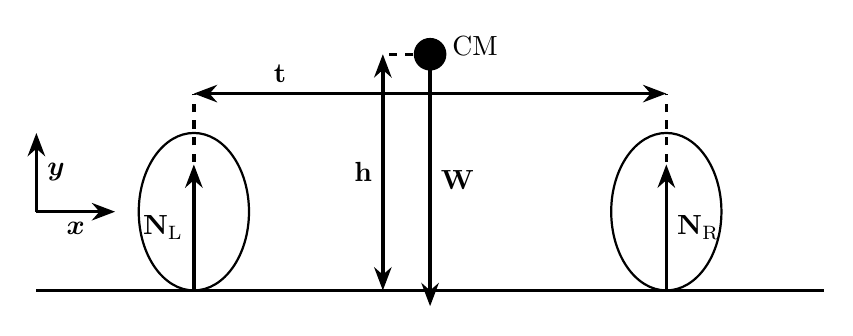
\begin{tikzpicture}[scale=2.0, >=Stealth, every node/.style={font=\normalsize}]
			
			% parameters
			\def\wheelsep{3.0}     % distance between wheel centers
			\def\wheeldia{0.9}     % wheel diameter
			\def\bodyh{1.0}        % rear body height above axle
			\def\axlepos{0.0}      % y position of axle/ground
			\def\cgx{0.0}          % horizontal offset of CG from midline (+ forward)
			\def\cgz{1.0}          % vertical position of CG above ground
			\def\wheelbigradius{0.5}
			
			% ground line
			\draw[thick] (-1,0) -- (\wheelsep+1,0);
			
			% wheel centers (two rear wheels)
			\coordinate (WL) at (0,0.5);
			\coordinate (WR) at (\wheelsep,0.5);
			
			% draw wheels
			%\draw[thick] (WL) circle[radius=0.5];
			%\draw[thick] (WR) circle[radius=0.5];
			\draw[thick] (WL) ellipse (0.35 and 0.5); 
			\draw[thick] (WR) ellipse (0.35 and 0.5); 
			
			
			% center of gravity (cg)
			\coordinate (CG) at ($(WL)!0.5!(WR) + (\cgx,\cgz)$);
			\draw[fill=black] (CG) circle (0.1);
			\node[right] at ($(CG)+(0.08,0.05)$) {CM};
			
			% weight
			\draw[very thick, ->] (CG) -- ++(0,-1.6) 
			node[midway,right] {$\mathbf{W}$};
			
			% normals
			\draw[very thick, ->] ($(WL)+(0,-\wheelbigradius)$) -- ++(0,0.8) 
			node[midway,left] {$\mathbf{N}_\text{L}$};
			\draw[very thick, ->] ($(WR)+(0,-\wheelbigradius)$) -- ++(0,0.8) 
			node[midway,right] {$\mathbf{N}_\text{R}$};
			
			% elipse
			\draw[very thick, <->] (0,2.5*\wheelbigradius) node[above right,xshift=25] {$\mathbf{t}$} -- (\wheelsep,2.5*\wheelbigradius) ;
			\draw[very thick, dashed, -] ($(WL)$) -- (0,2.5*\wheelbigradius);
			\draw[very thick, dashed, -] ($(WR)$) -- (\wheelsep,2.5*\wheelbigradius);
			
			\draw[very thick,dashed, -] (CG) -- ++(-0.3,0);
			\draw[very thick, <->] ($(CG)+(-0.3,0)$) -- (\wheelsep/2-0.3,0)
			node[midway, left] {$\mathbf{h}$};
			
			\draw[very thick, ->] ($(WL)+(-1,0)$) -- ++(0.5,0) 
			node[midway,below] {$\bm{x}$};
			\draw[very thick, ->] ($(WL)+(-1,0)$) -- ++(0,0.5) 
			node[midway,right] {$\bm{y}$};
		\end{tikzpicture}
		\caption{Schemat sił działających na samochód w stanie spoczynku (widok z tyłu).}
		\label{fig:stationary}
	\end{figure}
	
	\begin{figure}[h]
		\centering
		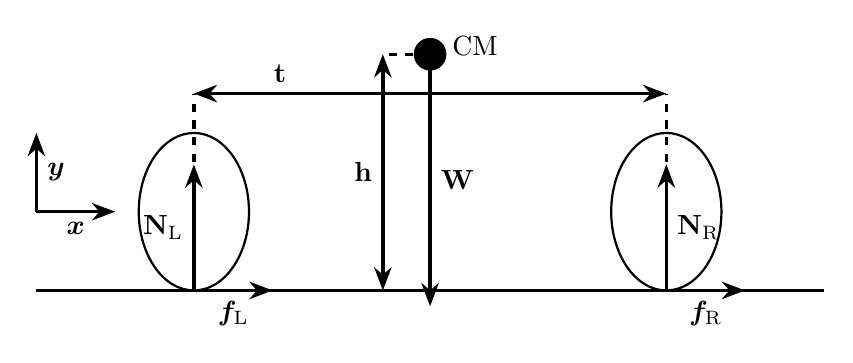
\begin{tikzpicture}[scale=2.0, >=Stealth, every node/.style={font=\normalsize}]
			
			% parameters
			\def\wheelsep{3.0}     % distance between wheel centers
			\def\wheeldia{0.9}     % wheel diameter
			\def\bodyh{1.0}        % rear body height above axle
			\def\axlepos{0.0}      % y position of axle/ground
			\def\cgx{0.0}          % horizontal offset of CG from midline (+ forward)
			\def\cgz{1.0}          % vertical position of CG above ground
			\def\wheelbigradius{0.5}
			
			% ground line
			\draw[thick] (-1,0) -- (\wheelsep+1,0);
			
			% wheel centers (two rear wheels)
			\coordinate (WL) at (0,0.5);
			\coordinate (WR) at (\wheelsep,0.5);
			
			% draw wheels
			%\draw[thick] (WL) circle[radius=0.5];
			%\draw[thick] (WR) circle[radius=0.5];
			\draw[thick] (WL) ellipse (0.35 and 0.5); 
			\draw[thick] (WR) ellipse (0.35 and 0.5); 
			
			
			% center of gravity (cg)
			\coordinate (CG) at ($(WL)!0.5!(WR) + (\cgx,\cgz)$);
			\draw[fill=black] (CG) circle (0.1);
			\node[right] at ($(CG)+(0.08,0.05)$) {CM};
			
			% weight
			\draw[very thick, ->] (CG) -- ++(0,-1.6) 
			node[midway,right] {$\mathbf{W}$};
			
			% normals
			\draw[very thick, ->] ($(WL)+(0,-\wheelbigradius)$) -- ++(0,0.8) 
			node[midway,left] {$\mathbf{N}_\text{L}$};
			\draw[very thick, ->] ($(WR)+(0,-\wheelbigradius)$) -- ++(0,0.8) 
			node[midway,right] {$\mathbf{N}_\text{R}$};
			
			% elipse
			\draw[very thick, <->] (0,2.5*\wheelbigradius) node[above right,xshift=25] {$\mathbf{t}$} -- (\wheelsep,2.5*\wheelbigradius) ;
			\draw[very thick, dashed, -] ($(WL)$) -- (0,2.5*\wheelbigradius);
			\draw[very thick, dashed, -] ($(WR)$) -- (\wheelsep,2.5*\wheelbigradius);
			
			\draw[very thick,dashed, -] (CG) -- ++(-0.3,0);
			\draw[very thick, <->] ($(CG)+(-0.3,0)$) -- (\wheelsep/2-0.3,0)
			node[midway, left] {$\mathbf{h}$};
			
			\draw[very thick, ->] ($(WL)+(0,-\wheelbigradius)$) -- ++(0.5,0) 
			node[midway,below] {$\bm{f}_\text{L}$};
			\draw[very thick, ->] ($(WR)+(0,-\wheelbigradius)$) -- ++(0.5,0) 
			node[midway,below] {$\bm{f}_\text{R}$};
			
			\draw[very thick, ->] ($(WL)+(-1,0)$) -- ++(0.5,0) 
			node[midway,below] {$\bm{x}$};
			\draw[very thick, ->] ($(WL)+(-1,0)$) -- ++(0,0.5) 
			node[midway,right] {$\bm{y}$};
		\end{tikzpicture}
		\caption{Schemat sił działających na samochód podczas skrętu w prawo (widok z tyłu).}
		\label{fig:turning}
	\end{figure}
	Ponieważ ciało nie porusza się w kierunku pionowym ($y$), bilans sił pionowych jest następujący:
	\begin{align}
		W=N_L+N_P
		\label{eq:y_equal}
	\end{align}
	gdzie $W = mg$ to całkowity ciężar, a $N_L$, $N_P$ to siły normalne po lewej i prawej stronie.
	
	Gdy samochód porusza się po zakrzywionej ścieżce, wymagana jest siła dośrodkowa:
	\begin{align}
		F_c=f_L+f_P
		\label{eq:centrifugal}
	\end{align}
	gdzie $f_L$ i $f_P$ to boczne siły opon. Wartość tej siły wynosi
	\begin{align}
		F_c = \frac{mv^2}{r} = ma_b
	\end{align}
	gdzie $a_b$ to przyspieszenie boczne. 
	Biorąc momenty względem środka masy, bilans momentów jest następujący:
	\begin{align}
		\tau_{SM}=Wr_{SM}+f_Lh+f_Ph+N_P\frac{w}{2}-N_L\frac{w}{2}
	\end{align}
	Ponieważ ciężar działa przez środek masy ($r_{SM}=0$) i zakładając, że pojazd się nie przewraca ($\tau_{SM}=0$), otrzymujemy:
	\begin{align}
		N_L = \frac{W}{2} + \frac{F_c h}{w}
	\end{align}
	Podstawiając $F_c = ma_b$ oraz $W=mg$ otrzymujemy:
	\begin{align}
		N_L = \frac{W}{2} + W \frac{a_b}{g}\frac{h}{w}
	\end{align}
	Definiując transfer obciążenia jako:
	\begin{align}
		\Delta W = W \frac{a_b}{g}\frac{h}{w}
	\end{align}
	obciążenia kóła lewego i prawego podczas skrętu w prawo stają się:
	\begin{empheq}[box=\fbox]{equation}
		N_L = \frac{W}{2} + \Delta W, \quad
		N_P = \frac{W}{2} - \Delta W
	\end{empheq}
	i zgodnie z symetrią, dla skrętu w lewo:
	\begin{empheq}[box=\fbox]{equation}
		N_L = \frac{W}{2} - \Delta W, \quad
		N_P = \frac{W}{2} + \Delta W
	\end{empheq}
	
	\subsection{Poślizg względny}
	Poślizg względny wyraża się wzorem:
	\begin{align}
		S=\frac{v_p}{v_{pgr}}
	\end{align}
	gdzie:
	\begin{itemize}
		\item $S$ - poślizg względny; $S=0$ brak poślizgu, $S=1$ pełny poślizg,
		\item $v_p$ - prędkość poślizgu koła
		\item $v_{pgr} $ - prędkość graniczna poślizgu koła
	\end{itemize}

	Ruch koła stanowi sumę ruchu postępowego z prędkością $v$ oraz ruchu obrotowego z prękością kątową $\omega$. Rysunek \ref{fig:toczenie_kol_sztywengo_bez_poslizgu} przestawia ruch koła sztywengo na sztywnej powierzchni bez poślizgu. W tym przypadku poślizg względnu nie wystepuje. Droga przebyta przez koło jest równa sumie obrotów wykonanych przez koło i wyraża się wzorem
	\begin{align}
		s=2\pi rn
	\end{align}
	\begin{figure}[h!]
		\centering
		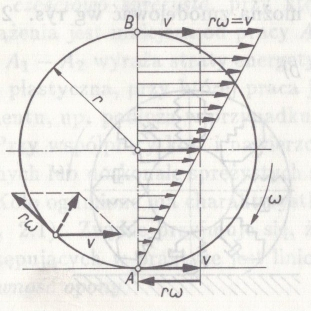
\includegraphics[scale=1.5]{toczenie_kola_sztywnego_bez_poslizgu.jpg}
		\caption{Toczenie się koła sztywnego bez poślizgu \cite{Arczynski}.}
		\label{fig:toczenie_kol_sztywengo_bez_poslizgu}
	\end{figure}
	W przypadku kiedy koło jest napędzane i występuje poślizg $\omega r > v$ przestawia to rysunek \ref{fig:toczenie_kol_sztywengo_z_poslizgiem_napedzanie}.
	Poślizg względny bedzie sie wyrażał wzorem
	\begin{align}
		S_n=\frac{v_p}{v_{pgr}}=\frac{v-r\omega}{-r\omega}=1-\frac{v}{r\omega}=1-\frac{r_t\omega}{r\omega}=1-\frac{r_t}{r}
	\end{align}
	\begin{figure}[h!]
		\centering
		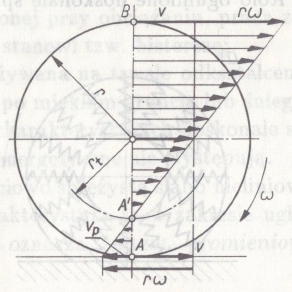
\includegraphics[scale=1.5]{toczenie_kola_sztywnego_z_poslizgiem_napedzanie.jpg}
		\caption{Toczenie się koła sztywnego z poślizgiem (napędzanie)  \cite{Arczynski}.}
		\label{fig:toczenie_kol_sztywengo_z_poslizgiem_napedzanie}
	\end{figure}
	Promień toczny przybiera wartości między zerem a $r$; gdy $r_t=0$, to $Sn=1$, gdy $r_t=r$, to $Sn=0$

	
	W przypadku kiedy koło jest hamowane i występuje poślizg $\omega r < v$ przestawia to rysunek \ref{fig:toczenie_kol_sztywengo_z_poslizgiem_hamowanie}.
	Poślizg względny bedzie sie wyrażał wzorem
	\begin{align}
		S_h=\frac{v_p}{v_{pgr}}=\frac{v-r\omega}{-r\omega}=1-\frac{v}{r\omega}=1-\frac{r\omega}{r_t\omega}=1-\frac{r}{r_t}
	\end{align}
		Promień toczny przybiera wartości między $r$ a nieskończonością; gdy $r_t=r$, to $Sn=0$, gdy $r_t=\infty$, to $Sn=0$
	\begin{figure}[h!]
		\centering
		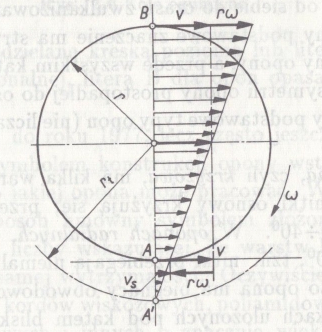
\includegraphics[scale=1.5]{toczenie_kola_sztywnego_z_poslizgiem_hamowanie.jpg}
		\caption{Toczenie się koła sztywnego z poślizgiem (hamowanie)  \cite{Arczynski}.}
		\label{fig:toczenie_kol_sztywengo_z_poslizgiem_hamowanie}
	\end{figure}
	
	Znająć przebytą drogę koła $s$ oraz liczbę jego obrotów $n$ można wyznaczyć dla obu poślizgów promień toczenia $r_t$
	\begin{align}
		r_t=\frac{s}{2\pi n} 
	\end{align}
	a stąd poślizg.
	Poślizg koła idealnie sztywnego można przyjąć jako dobre przybliżenie poślizgu koła częsciowo sprężystego.
	\subsection{Przyczepność opon}
	
	Siłę przyczepności opony można wyrazić jako:
	\begin{align}
		F \leq \mu N = \sqrt{X^2 + Y^2}
	\end{align}
	
	gdzie:
	\begin{itemize}
		\item $\mu$ to współczynnik przyczepności,
		\item $N$ to siła normalna (ciężar działający na oponę),
		\item $X$ to siła podłużna,
		\item $Y$ to siła boczna.
	\end{itemize}
	% Optional TikZ diagram for illustration:
	\begin{figure}[h]
		\centering
		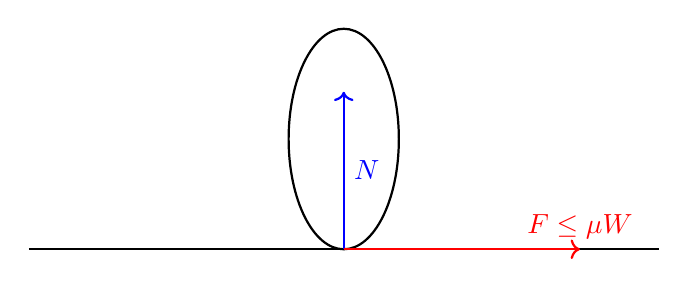
\begin{tikzpicture}[scale=2]
			% Road
			\draw[thick] (-2,0) -- (2,0);
			% Tire
			\draw[thick] (0,0.7) ellipse (0.35 and 0.7);
			% Normal force
			\draw[->, thick, blue] (0,0.0) -- (0,1) node[midway,right] {$N$};
			% Friction force
			\draw[->, thick, red] (0,0.0) -- (1.5,0.0) node[right,above] {$F \leq \mu W$};
		\end{tikzpicture}
		\caption{Forces acting on a tire in contact with the road.}
	\end{figure}
	
	Prawa strona nierówności reprezentuje maksymalną siłę napędową lub hamującą, którą można przenieść bez poślizgu. Jeśli ten limit zostanie przekroczony, opona przechodzi od tarcia statycznego do kinetycznego, co skutkuje utratą przyczepności \cite{Arczynski}.
	
	W praktyce współczynnik przyczepności $\mu$ nie jest stały. Zależy od wielu czynników, w tym:
	\begin{itemize}
		\item Odkształcenia opony i wzoru bieżnika,
		\item Temperatury opony i nawierzchni drogi,
		\item Warunków pogodowych (sucho, mokro, lód, śnieg),
		\item Ciśnienia w oponach,
		\item Tekstury nawierzchni i jej zanieczyszczeń (kurz, olej, żwir itp.).
	\end{itemize}
	
	Dobrze zaprojektowana opona zapewnia płynne przejście między tarciem statycznym a kinetycznym, tak aby przyczepność nie została utracona nagle, co jest kluczowe dla stabilności i bezpieczeństwa pojazdu. 
	
		\subsection{Oznaczenia opon F1}
	
	Od 2022 roku bolidy F1 korzystają z sześciu typów opon na suchą nawierzchnię, oznaczonych od C0 do C5, gdzie C0 są najtwardsze, a C5 najmiększe. Dodatkowo dostępne są dwa typy opon na mokrą nawierzchnię: opony przejściowe, używane, gdy na torze nie ma stojącej wody, oraz opony deszczowe, stosowane podczas intensywnych opadów.  
	
	Rysunek \ref{fig:tires_dry} przedstawia opony do suchej nawierzchni, natomiast rysunek \ref{fig:tires_wet} – do nawierzchni mokrej.
	
	Wymiary opon bolidów F1 podawane są w formacie: \textit{W/D-O} gdzie:
	\begin{itemize}
		\item $W$ – szerokość opony [mm],
		\item $D$ – średnica opony [mm],
		\item $O$ – średnica obręczy koła [cale].
	\end{itemize}
	
	Dla bolidów F1 wymiary opon prezentują się następująco: przednie opony mają wymiary \textit{305/720-18}, a tylne \textit{405/720-18}.
	
	\begin{figure}[h!]
		\centering
		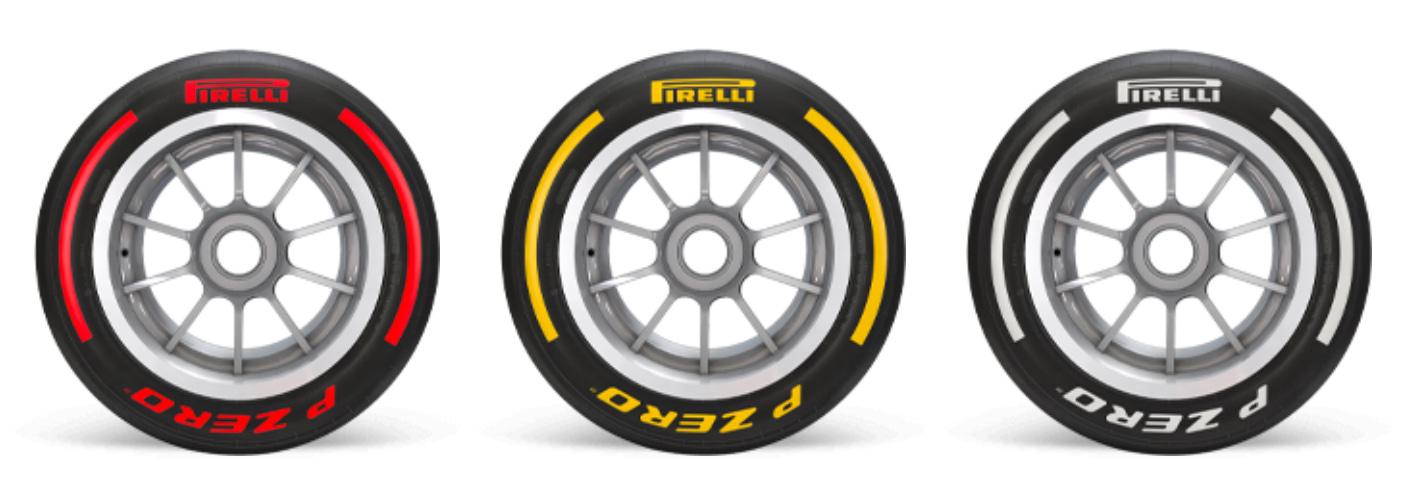
\includegraphics[scale=0.25]{dry_tires.jpg}
		\caption{Opony przeznaczone do warunków suchych (od lewej C0) \cite{tires}.}
		\label{fig:tires_dry}
	\end{figure}
	
	\begin{figure}[h!]
		\centering
		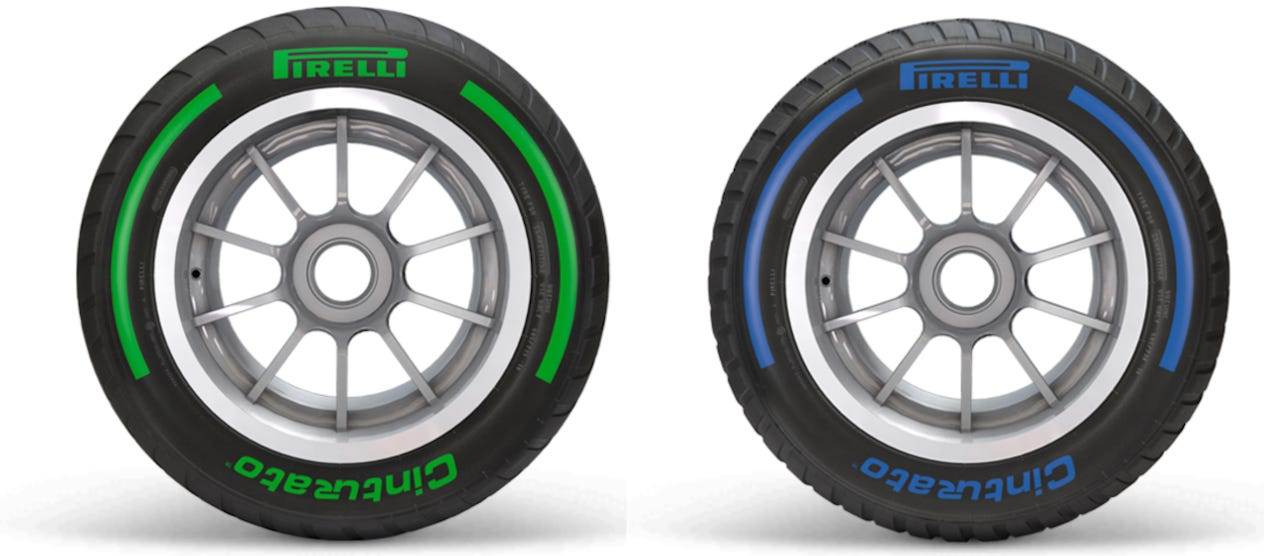
\includegraphics[scale=0.25]{wet_tires.jpg}
		\caption{Opony przeznaczone do warunków mokrych (od lewej opony przejściowe) \cite{tires}.}
		\label{fig:tires_wet}
	\end{figure}
	
	\subsection{Siły reakcji nawierzchni}
	Siły działające na koła przedstawia się jako sumę sił oddziałujących na oba koła danej osi. Łączna wartość tych sił nazywana jest naciskiem osi. Rozważmy samochód stojący na powierzchni pochyłej (rysunek \ref{fig:rozklad_sil_pojazd}).
	\begin{figure}[h!]
		\centering
		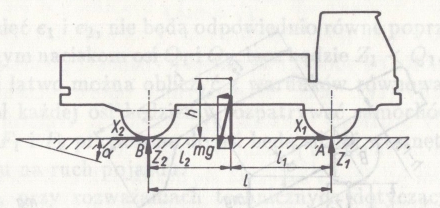
\includegraphics{rozklad_sil_pojazd.jpg}
		\caption{Samochód stojący na nawierzchni pochyłej \cite{Arczynski}.}
		\label{fig:rozklad_sil_pojazd}
	\end{figure}
	Z równań momentów względem punktów styku otrzymujemy:
	\begin{align}
		Z_1=\frac{mg}{l}(l_2\cos \alpha -h\sin \alpha)\\
		Z_2=\frac{mg}{l}(l_1\cos \alpha +h\sin \alpha)
	\end{align}
	
	\section{Opory ruchu}
	Podczas analizy ruchu pojazdu przyjmuje się następujące uproszczenia:
	\begin{figure}[h!]
		\centering
		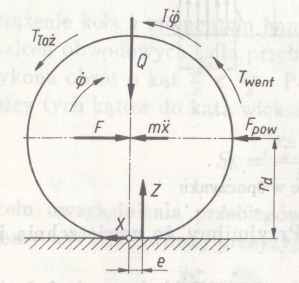
\includegraphics{rozklad_kolo_toczone.jpg}
		\caption{Rozkład sił i momentów działających na koło toczne \cite{Arczynski}.}
		\label{fig:rozklad_kolo_toczone}
	\end{figure}
	\begin{itemize}
		\item pomija się przesunięcie normalnej reakcji $Z$ (rys. \ref{fig:rozklad_kolo_toczone}), ponieważ błąd przy zwykłych pojazdach nie przekracza 1\%,
		\item nie uwzględnia się transferu ciężaru przy przyspieszeniu – jednak w przypadku bolidów należy to brać pod uwagę ze względu na znacznie większe przyspieszenia niż w samochodach standardowych,
		\item nie rozpatruje się oddzielnie oporów toczenia poszczególnych opon, lecz ich sumę.
	\end{itemize}
	Aby pojazd poruszał się ruchem jednostajnym prostoliniowym, musi być spełniony warunek:
	\begin{align}
		F_n-\sum F_{op}=0
	\end{align}
	gdzie:
	\begin{align}
		\sum F_{op}=F_t+F_p+F_w+F_b+F_s
	\end{align}
	Odpowiadają one kolejno siłom oporu: toczenia, powietrza, wzniesienia, bezwładności i skrętu.
	
	\subsection{Siła oporu toczenia}
	Siłę oporu toczenia przyjmuje się jako sumę oporów wszystkich opon:
	\begin{align}
		F_t=mgf
	\end{align}
	gdzie $f$ oznacza współczynnik oporu toczenia.  
	Współczynnik $f$ można zapisać wzorem:
	\begin{align}
		f=f_0(1+AV^2)
	\end{align}
	gdzie:
	\begin{itemize}
		\item $A$ – współczynnik zależny od nawierzchni: od $4.5\cdot10^{-5}$ dla dróg gładkich do $10\cdot 10^{-5}$ dla dróg wyboistych; dla nawierzchni asfaltowych i betonowych można przyjąć $A=5\cdot 10^{-5}$,
		\item $V$ – prędkość liniowa pojazdu.
	\end{itemize}
	
	\subsection{Siła oporu powietrza}
	\begin{figure}[h!]
		\centering
		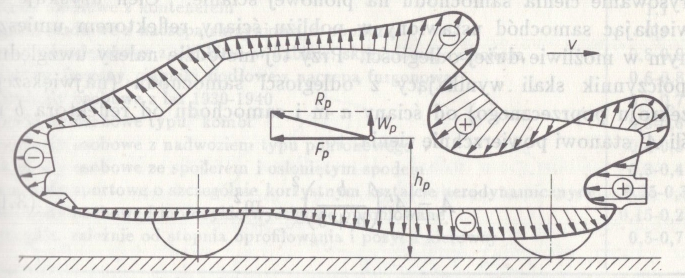
\includegraphics{rozklad_sil_powietrza.jpg}
		\caption{Rozkład ciśnień powietrza na powierzchni samochodu \cite{Arczynski}.}
		\label{fig:rozklad_sil_powietrza}
	\end{figure}
	Siłę oporu aerodynamicznego opisuje równanie:
	\begin{align}
		F_p=\frac{1}{2}\gamma v^2Ac_x
	\end{align}
	gdzie:
	\begin{itemize}
		\item $\gamma$ – gęstość powietrza (zależna od temperatury i wilgotności),
		\item $A$ – powierzchnia czołowa pojazdu,
		\item $c_x$ – współczynnik oporu aerodynamicznego,
		\item $v$ – prędkość względna pojazdu względem powietrza.
	\end{itemize}
	W praktyce powierzchnię czołową bolidów lub wartość całkowitego współczynnika oporu można znaleźć w źródłach i wtedy równanie upraszcza się do:
	\begin{align}
		F_p=\frac{1}{2}kv^2
	\end{align}
	Przez prędkość względną rozumiemy prędkość pojazdu względem wiatru. Przy jeździe pod wiatr prędkość względna rośnie, natomiast z wiatrem maleje. W przypadku wiatru bocznego prędkości dodają się wektorowo. Wiatr boczny działa na pojazd siłą, która może wywołać moment obrotowy wpływający na sterowność pojazdu. W takich sytuacjach należy uwzględnić współczynnik aerodynamiczny $c_y$ oraz powierzchnię boczną $Y$.
	
	Przy modelowaniu bolida również istotne jest uwzględnienie siły nośniej naporu $W_p$ oraz docisk aerodynamiczny.
	
	Przy modelowaniu bolida istotne jest również uwzględnienie \textbf{siły nośnej naporu} $W_p$ oraz \textbf{docisku aerodynamicznego}, które znacząco wpływają na przyczepność kół i zachowanie pojazdu przy dużych prędkościach.
	\subsection{Siła oporu wzniesienia}
	Siła oporu wzniesienia przyjmuje wartości dodatnie, gdy pojazd jedzie pod górę, oraz ujemne, gdy zjeżdża w dół. Na rysunku \ref{rozklad_sil_wzniesienie} przedstawiono przypadek wjazdu pod górę.
	\begin{figure}[h!]
		\centering
		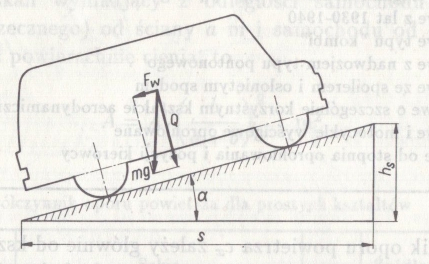
\includegraphics{rozklad_sil_wzniesienie.jpg}
		\caption{Opór wzniesienia \cite{Arczynski}.}
		\label{fig:rozklad_sil_wzniesienie}
	\end{figure}
	\begin{align}
		F_w=mg\sin \alpha
	\end{align}
	Dla wzniesień do $12^{\circ}$ można przybliżać $\sin \alpha$ przez $\tan \alpha$, gdzie:
	\begin{align}
		\tan \alpha = \frac{h_s}{s}
	\end{align}
	(błąd wynosi do ok. 2\%). Wówczas wzór przyjmuje postać:
	\begin{align}
		F_w=mg\frac{h_s}{s}
	\end{align}
	
	\subsection{Siła oporu bezwładności}
	Trza zrobić ale to trudne
	\subsection{Siła oporu skrętu}
	\begin{align}
		F_s=mgf_s
	\end{align}
	tu też trzeba coś dopisać
	\bibliographystyle{apalike}
	\bibliography{refs} 
\end{document}

